%
% k-schwarzschild.tex
%
% (c) 2017 Prof Dr Andreas Müller, Hochschule Rapperswil
%
\chapter{Schwarzschild-Metrik und schwarze Löcher%
\label{skript:chapter:schwarzschild}}
\lhead{Schwarzschild-Metrik}
\rhead{}
Die Einsteinschen Feldgleichungen schränken die Metriken ein,
die in einem Raumzeit-Gebiet über\-haupt möglich sind.
Damit stellt sich automatisch die Frage, wie die Einsteinsche Theorie 
das Gravitationsfeld in der Umgegung eines Sterns beschreiben kann.
Schon wenige Monate nachdem Einstein seine allgemeine Relativitätstheorie
veröffentlich hat, hat Karl Schwarzschild eine Lösung der Einsteinschen
Feldgleichungen gefunden.
Daraus lassen sich die Bewegungsgleichungen eines Körpers in der Nähe
eines Sterns ableiten und es sollte möglich sein, den Unterschied zwischen
der Newtonschen Gravitations-Theorie und Einsteinschen  zu quantifizieren
und damit Tests der allgmeinen Relativitätstheorie zu ermöglichen.

\section{Eine kugelsymmetrische, statische Lösung}
\rhead{Schwarzschild-Metrik}
Karl Schwarzschild suchte eine Metrik, die sich mit der Zeit nicht ändert,
also
\[
\frac{\partial g_{\mu\nu}}{\partial t}=0,
\]
und die ausserdem kugelsymmetrisch sein soll.
Diese Metrik sollte eine erste Approximation für die Gravitation in
der Umgebung eines Sterns sein.
Natürlich berücksichtigt dieses Modell weder, dass sich Sterne mit
der Zeit entwickeln, noch die Tatsache, dass sich Sterne normalerweise
um eine Achse drehen, dass man also gar nicht eine rotationssymmetrische
Lösung erwarten darf.

Die Längenmessung
\begin{equation}
ds^2
=
-c^2\,dt^2 + dr^2 + r^2 d\Omega^2
\qquad
d\Omega^2 = d\vartheta^2 + \sin^2\vartheta\,d\varphi^2
\label{skript:kruemmung:euklid}
\end{equation}
im Raum mit Kugelkoordinaten ist natürlich eine solche Metrik,
doch da dies nur eine andere Parametrisierung des euklidischen
Raumes ist, ist diese Geometrie flach.
Sie kann also sich nicht ein Modell eines Sternes sein.

Man kann eine Lösung der Feldgleichungen finden, indem man den
einzelnen Termen der euklischen Metrik~\eqref{skript:kruemmung:euklid}
zunächst unbestimmte Faktoren hinzufügt, die nur von $r$ abhängt,
und dann mit Hilfe der Feldgleichungen dafür Differentialgleichungen
herleitet.
Wir wollen diesen beschwerlichen Weg nicht gehen, und uns mit dem
Resultate zufriedenstellen, es lautet
\begin{equation}
ds^2
=
-\biggl(1-\frac{r_g}r\biggr)c^2\,dt^2
+\frac1{\displaystyle 1-\frac{r_g}r}\,dr^2 + r^2\,d\Omega^2.
\label{skript:kruemmung:schwarzschildmetrik}
\end{equation}
Man kann nachrechnen, zum Beispiel mit Hilfe der früher vorgestellen
Maxima-Programme, dass der Einstein-Tensor für diese Metrik überall
verschwindet.

\section{Der Fall $r=r_g$}
\rhead{Der Fall $r=r_g$}
Es scheint, dass die Metrik für $r=r_g$ nicht wohldefiniert ist,
da dann der Nenner im zweiten Term nicht wohldefiniert ist.
Dem ist jedoch nicht so, wie man durch Wahl eines anderen Koordinatensystems
zeigen kann.
Wir ersetzen die Zeitkoordinaten $t$ durch $\tau$, und die $r$-Koordinate
durch $R$ mit der vorläufig noch unbestimmten Funktion $f(r)$.
Es soll gelten
\begin{equation}
\begin{aligned}
c\tau
&=
ct + \int\frac{f(r)\,dr}{\displaystyle 1-\frac{r_g}{r}}
&
&\text{und}
&
R
&=
ct
+
\int\frac{dr}{\displaystyle \biggl(1-\frac{r_g}{r}\biggr)f(r)}
\end{aligned}
\label{skript:kruemmung:finkelsteindefinition}
\end{equation}
mit einer vorläufig noch unbestimmten Funktion $f(r)$.
Die Integrationskonstante in den beiden unbestimmten Integralen
entspricht einer Wahl des $t$- bzw.~$\tau$-Nullpunktes und ist
daher nicht von Bedeutung.
Um die Metrik in $\tau$ und $R$ ausdrücken zu können, müssen wir 
den Zusammenhang zwischen $dr$, $dR$, $dt$ und $d\tau$ kennen.
Wir finden diesen durch Ableiten der beiden Definitionsgleichungen
\eqref{skript:kruemmung:finkelsteindefinition}:
\begin{align*}
c\,d\tau
&=
c\,dt + \frac{f(r)}{\displaystyle 1-\frac{r_g}{r}}\,dr,
\\
dR
&=
c\,dt
+
\frac{1}{\displaystyle\biggl(1-\frac{r_g}{r}\biggr)f(r)}\,dr.
\end{align*}
Für die Schwarzschild-Metrik brauchen wir die Quadrate davon:
\begin{align*}
c^2\,d\tau ^2
&=
c^2\,dt^2 + 2\frac{cf(r)}{\displaystyle 1-\frac{r_g}{r}}\,dt\,dr
+\frac{f(r)^2}{\biggl(\displaystyle 1-\frac{r_g}{r}\biggr)^2}\,dr^2,
\\
dR^2
&=
c^2\,dt^2 + 2\frac{c}{\displaystyle\biggl(1-\frac{r_g}{r}\biggr)f(r)}\,dt\,dr
+
\frac{1}{\displaystyle \biggl(1-\frac{r_g}{r}\biggr)^2f(r)^2}\,dr^2.
\end{align*}
Wir müssen diese beiden Ausdrücke so kombinieren, dass der gemischte
Term $dt\,dr$ wegfällt, denn dieser kommt in der Schwarzschild-Metrik
nicht vor.
Dazu multiplizieren wir die zweite Zeile mit $f(r)^2$, und subtrahieren.
Wir erhalten
\begin{equation}
c^2\,d\tau^2 - f(r)^2\,dR^2
=
(1-f(r)^2)c^2\,dt^2
+\frac{f(r)^2-1}{\displaystyle\biggl(1-\frac{r_g}{r}\biggr)^2}\,dr^2.
\end{equation}
Damit daraus die Schwarzschild-Metrik wird, müssen wir vor dem $dt^2$
Term einen Faktor der Form $(1-r_g/r)$ haben, wir müssen also zunächst
alles durch $1-f(r)^2$ dividieren, und dann mit $1-r_g/r$ multiplizieren.
Wir kehren ausserdem das Vorzeichen und erhalten
\[
\frac{\displaystyle 1-\frac{r_g}{r}}{1-f(r)^2}
(-c^2\,d\tau^2 + f(r)^2\,dR^2)
=
-\biggl(1-\frac{r_g}{r}\biggr)c^2\,dt^2
+\frac{1}{\displaystyle 1-\frac{r_g}{r}}\,dr^2
\]
Bis auf die Terme $d\Omega^2$ steht auf der rechten Seite die
Schwarzschild-Metrik.
Von den Termen auf der linken Seite ist nur der Bruch
\[
\frac{\displaystyle 1-\frac{r_g}{r}}{1-f(r)^2}
\]
problematisch, allerdings nur, wenn der Nenner $1-f(r)^2$ eine
Nullstelle hat.
Wir können den ganzen Bruch zum Verschwinden bringen, indem wir die
Wahlmöglichkeiten für $f(r)$ ausnützen und 
\[
f(r)=\sqrt{\frac{r_g}{r}}
\]
wählen.
Setzen wir dies ein, erhalten wir die Metrik in $\tau$-$R$-Koordinaten
jetzt in der Form
\begin{equation}
ds^2
=
-c^2\,d\tau^2 + \frac{r_g}{r}\,dR^2 + r^2 d\Omega^2,
\label{skript:kruemmung:finkelstein}
\end{equation}
aber natürlich müssen wir $r$ und $r^2$ ebenfalls durch die Koordinaten
$\tau$ und $R$ ausdrücken.

Da jetzt $f(r)$ bekannt ist, können wir die
Integrale~\eqref{skript:kruemmung:finkelsteindefinition} auswerten.
Wir berechnen
\begin{align*}
R-c\tau
&=
\int\frac{dr}{\displaystyle \biggl(1-\frac{r_g}{r}\biggr)f(r)}
- \int\frac{f(r)\,dr}{\displaystyle 1-\frac{r_g}{r}}
=
\int\frac{1-f(r)^2}{\displaystyle\biggl(1-\frac{r_g}{r}\biggr) f(r)}\,dr
=
\int\frac{1}{f(r)}\,dr
=
\frac{1}{\sqrt{\mathstrut r_g}}\int\sqrt{\mathstrut r}\,dr
\\
&=
\frac{1}{\sqrt{\mathstrut r_g}} \frac{2}{3}r^{\frac{3}{2}}
\end{align*}
Damit kann man jetzt $r$ durch $R-c\tau$ ausdrücken
\begin{equation}
r
=
\biggl(\frac{3}{2}(R-c\tau)r_g^{\frac{1}{2}}\biggr)^{\frac23}
=
\biggl(\frac{3}{2}(R-c\tau)\biggr)^{\frac23} r_g^{\frac13}
\label{skript:kruemmung:finkelsteinr}
\end{equation}
Der $r$-Koordinate $r_g$ entspricht jetzt die Gerade
\[
R-c\tau = \frac23 r_g = R_g.
\]
Setzen wir dies in die Metrik~\eqref{skript:kruemmung:finkelstein}
ein, erhalten wir
\[
ds^2
=
-c^2 \,d\tau^2
+r_g^{\frac23}\biggl(\frac32(R-c\tau)\biggr)^{-\frac23}\,dR^2
+ r_g^{\frac23}\biggl(\frac32(R-c\tau)\biggr)^{\frac43}\,d\Omega^2.
\]
Es ist klar, dass in diesen Koordinaten in keinem Term für $r=r_g$
eine Singularität auftritt.
Die hier berechneten Koordinaten $\tau$ und $R$ heissen
Finkelstein-Koordinaten.

\section{Absturz ins Zentrum}
\rhead{Absturz ins Zentrum}
\begin{figure}
\centering
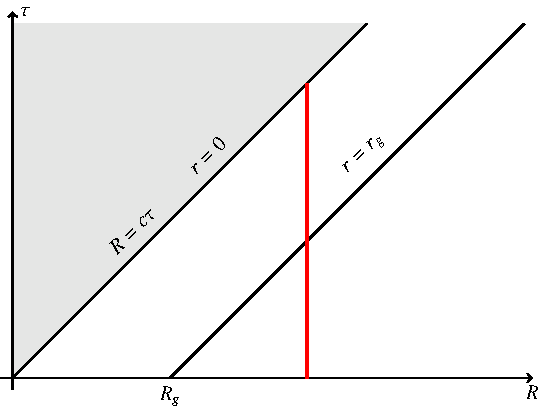
\includegraphics{chapters/tikz/absturz.pdf}
\caption{Radialer Absturz eines Teilchens (rote Bahn) in einem Zentralfeld
in Finkelstein-Koordinaten.
Das Teilchen stürzt in endlicher Eigenzeit ins Zentrum.
\label{skript:kruemmung:fig:absturz}}
\end{figure}
\begin{figure}
\centering
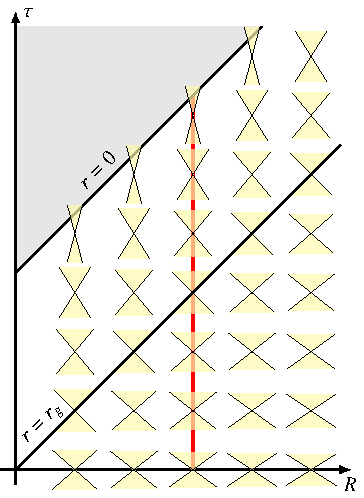
\includegraphics{chapters/tikz/lichtkegel.pdf}
\caption{Lichtkegel in Finkelstein-Koordinaten.
\label{skript:kruemmung:fig:lichtkegel}}
\end{figure}
In Finkelstein-Koordinaten verschwindet die Singularität bei $r=r_g$,
es sollte daher auch einfacher werden, die Bahn eines radial ins
Zentrum des Feldes stürzenden Teilchens zu berechnen.
Dazu können wir die Winkel-Koordinaten $\vartheta$ und $\varphi$
vernachlässigen, und nur mit den Koordinaten $\tau$ und $R$ und der
Metrik
\[
ds^2
=
-c^2 \,d\tau^2
+r _g^{\frac23}\biggl(\frac32(R-c\tau)\biggr)^{\frac23}\,dR^2
\]
arbeiten.
Zur Berechnung der Bahnkurven brauchen wir die Christoffel-Symbole
2.~Art.
Die Berechnung mit Maxima ergibt
\begin{align*}
\Gamma^1_{11} &= 0,&
\Gamma^1_{12} &= 0,&
\Gamma^1_{21} &= 0,&
\Gamma^1_{22} &= \frac{2^{\frac23}r_g^{\frac23}}{(3(R-c\tau))^{\frac53}},\\
\Gamma^2_{11} &= 0,&
\Gamma^2_{12} &= \frac1{3(R-c\tau)},&
\Gamma^2_{21} &= \frac1{3(R-c\tau)},&
\Gamma^2_{22} &= -\frac1{3(R-c\tau)}.
\end{align*}
Wir beschreiben die Bahn eines Teilchens welches sich in diesem Feld
radial bewegt mit den Funktionen $\tau(s)$ und $R(s)$.
Wir untersuchen ein Teilchen, welches beim Punkt $\tau(0)=0$ und $R(0)=R_0$
mit Anfangsrichtung $\dot\tau(0)=1$ und $\dot R(0)=0$ in das Gravitationsfeld
stürzt.
Die Geodätengleichungen lauten
\begin{align*}
\frac{d^2\tau(s)}{ds^2}
&=
\Gamma^1_{22}\biggl(\frac{dR(s)}{ds}\biggr)^2,
\\
\frac{d^2R(s)}{ds^2}
&=
\Gamma^2_{12}\frac{d\tau(s)}{ds}\frac{dR(s)}{ds}
+
\Gamma^2_{22}\biggl(\frac{dR(s)}{ds}\biggr)^2.
\end{align*}
Da für die Anfangsbedinung $\dot R=0$ ist und auf der rechten Seite
$\dot R$ in jedem Term vorkommt, folgt aus der zweiten Gleichung
$\ddot R=0$, $\dot R$ kann sich also nicht ändern.
Wenn aber $\dot R=0$ für alle Werte von $s$, dann ist nach der ersten
Gleichung auch $\ddot \tau=0$ und damit $\dot \tau=1$.
Die Lösungskurve ist also $R=R_0$ und $\tau=s$, rot dargestellt in
Abbildung~\ref{skript:kruemmung:fig:absturz}.

Mit Hilfe der Formel~\eqref{skript:kruemmung:finkelsteinr}
kann man damit auch $r$ für den radialen Absturz angeben:
\[
r(\tau)=\biggl(\frac32(R_0-c\tau)\biggr)^{\frac23}r_g^{\frac13}.
\]

\section{Ereignishorizont%
\label{skript:section:ereignishorizont}}
\rhead{Ereignishorizont}
Wir betrachten wieder die
Schwarzschild-Metrik~\eqref{skript:kruemmung:schwarzschildmetrik}
und möchten genauer verstehen, was bei $r=r_g$ passiert.
Dazu überlegen wir uns, wie ein Geodäte eines realen Teilchens 
aussieht.
Wir wissen, dass reale Teilchen sich so bewegen müssen, dass der
Tangentialvektor negative Metrik hat.
Ein Teilchen in Ruhe hat zum Beispiel $\dot r=0$, $\dot \vartheta=0$ und
$\dot varphi=0$, einzig $\dot t\ne 0$.
Da der Koeffizient von $dt^2$
\[
-\biggl(1-\frac{r_g}{r}\biggr)
\quad
\begin{cases}
<0&\qquad r > r_g
\\
>0&\qquad r < r_g
\end{cases}
\]
für $r>r_g$
negativ ist folgt, dass es tatsächlich möglich ist, dass sich ein Teilchen
in festem Abstand vom Zentrum aufhalten kann.
Sobald aber $r<r_g$ ist, ist der Koeffizient von $dt^2$ positiv,
fester Abstand vom Zentrum ist nicht mehr möglich.

Für $r<r_g$ wechselt aber auch das Vorzeichen des Koeffizienten
\[
\frac1{\displaystyle1-\frac{r_g}{r}}
\quad
\begin{cases}
>0&\qquad r>r_g
\\
<0&\qquad r<r_g
\end{cases}
\]
von $dr^2$, damit wird plötzlich der Vektor $\dot t=0$, $\dot r\ne 0$,
$\dot\vartheta=\dot\varphi=0$ zeitartig.
Sobald ein Teilchen sich innerhalb des Radius $r_g$ befindet, kann
sein Radius nur noch abnehmen.
Die Berechnung der Bahn eines solchen Teilchens zeigt auch, dass
es unausweichlich in endlicher Zeit ins Zentrum stürzen wird.

\begin{figure}
\centering
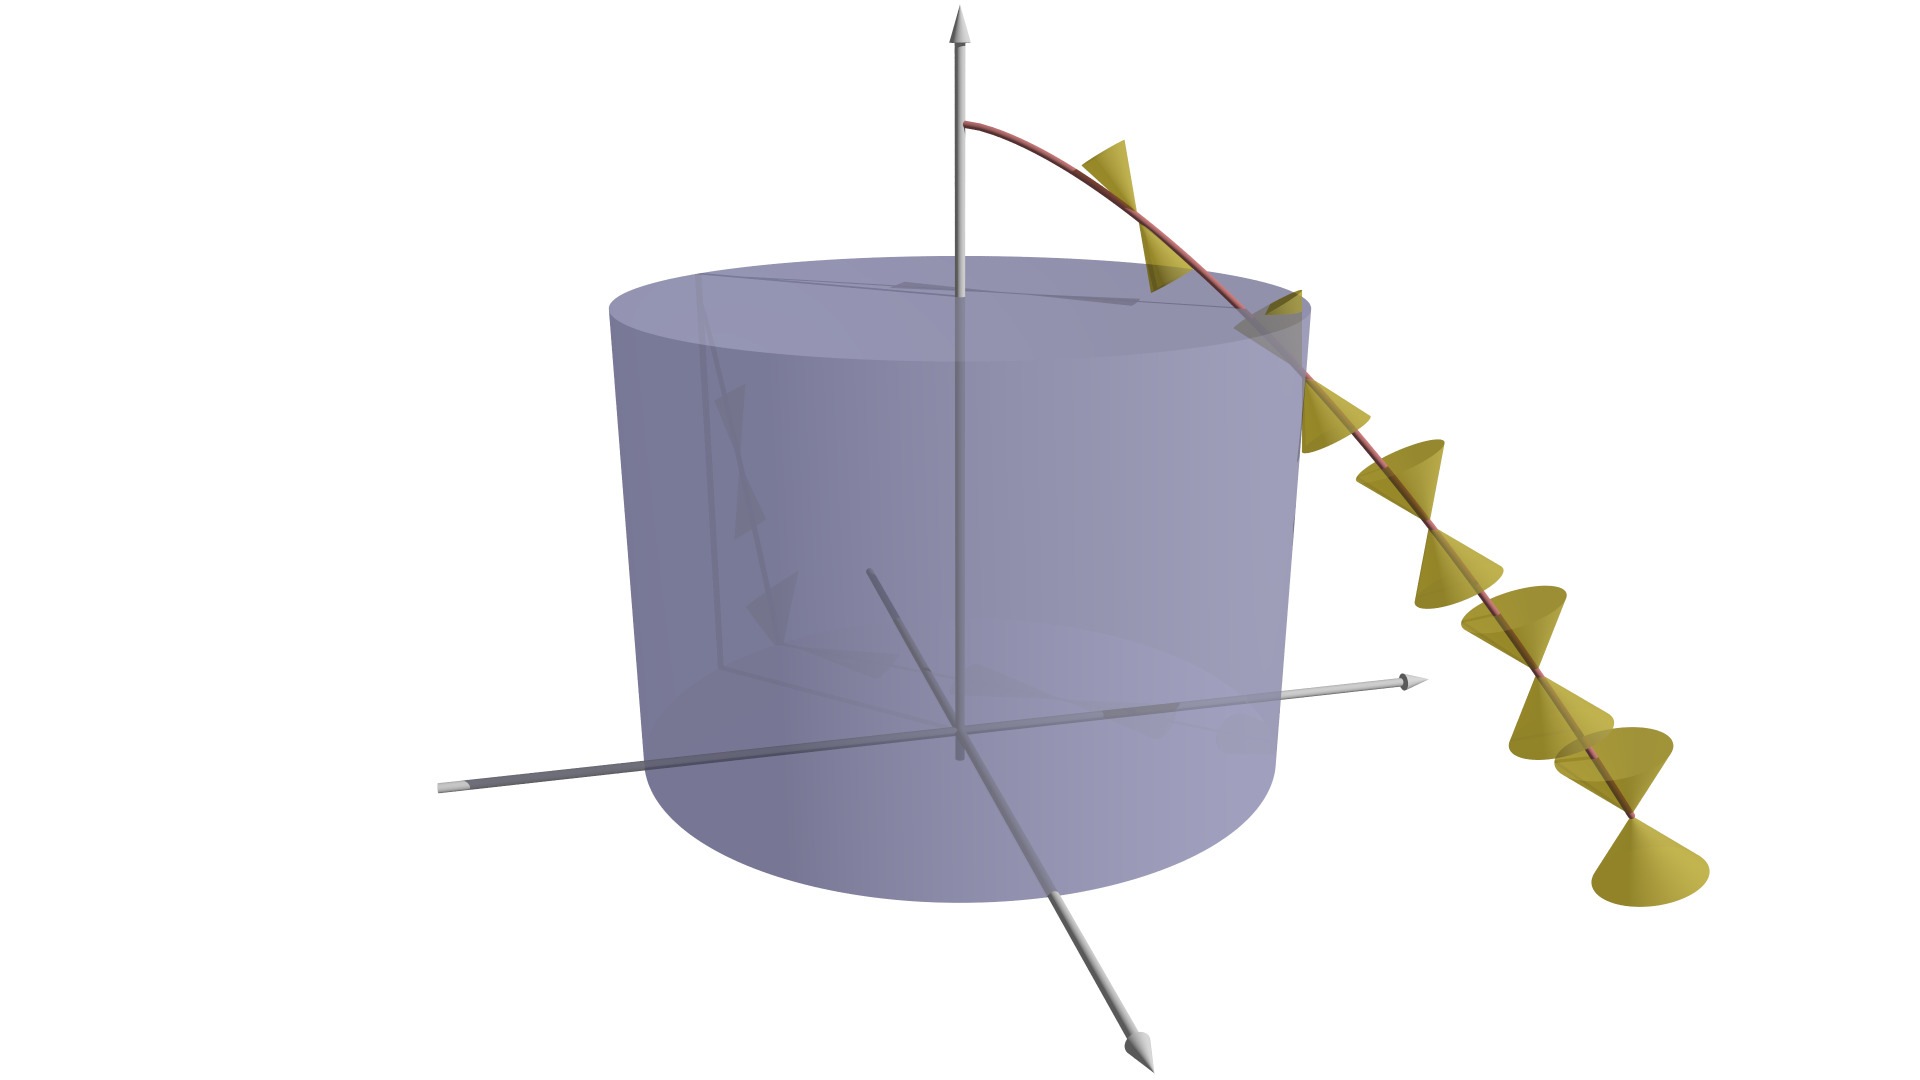
\includegraphics[width=\hsize]{chapters/3d/blackhole.jpg}
\caption{Absturz eines Teilchens durch den Ereignishorizont in
$(\tau,r,\varphi)$-Koordinaten.
Sobald das Teilchen durch den Ereignishorizont gefallen ist,
befindet sich der ganze zukünftige Lichtkegel eines Teilchens 
immer vollständig im inneren des Gebietes $r<r_g$.
\label{skript:kruemmung:fig:blackhole}}
\end{figure}


\section{Was spürt man am Ereignishorizont?%
\label{skript:section:wasspuertman}}
\rhead{Was spürt man am Ereignishorizont?}
Der Riemannsche Krümmungstensor gibt an, wie schnell Geodäten von Teilchen
wegen unterschiedlicher Gravitationswirkung sich voneinander entfernen.
Er bestimmt also die Gezeitenkräfte, die ein Astronaut spürt, der in
diesem Gravitationsfeld abstürzt.
die Gezeitenkräfte, die ein Astronaut spürt, der in
diesem Gravitationsfeld abstürzt.
Die Berechnung des Riemann-Tensors mit Maxima ergibt aber:
\begin{align*}
R_{1212}&=-\frac{r_g}{r^3},
\end{align*}
die Gezeitenkräfte in radialer Richtung werden für den Astronauten
also zwar immer grösser, aber bei $r=r_g$ spürt er nichts besonderes.

\section{Bedeutung von $r_g$}
\rhead{Bedeutung von $r_g$}
In Abschnitt~\ref{skript:section:ereignishorizont} haben wir gefunden,
dass sich bei der Koordinaten $r=r_g$ der Ereignishorizont befindet.
Es ist auch einigermassen klar, dass dieser Radius $r_g$ mit der
Masse des Objektes zusammenhängen muss.
Doch wie gross ist eiegentlich der Gravitations-Radius $r_g$ verschiedener
uns umgebender Himmelskörper? Kann es überhaupt einen Körper geben, der
so dicht ist, dass er kleiner ist als sein Gravitationsradius?

In grosser Entfernung $r \gg r_g$ vom Zentrum ist die Metrik fast flach,
das Feld ist dort sehr schwach.
Durch Vergleich mit der Näherung~\eqref{skript:gravitation:naeherung}
finden wir
\[
\frac{r_g}{r} = \frac{2MG}{r},
\qquad\Rightarrow\qquad
r_g=\frac{2MG}{c^2}
\]
Der Radius $r_g=2MG$ heisst der {\em Gravitationsradius} oder 
\index{Gravitationsradius}
{\em Schwarzschild-Radius}.
\index{Schwarzschild-Radius}
Der numerische Zusammenhang zwischen Masse und Gravitationsradius
in SI-Einheiten ist
\[
r_g = \frac{2G}{c^2}M
=
2\cdot 6.67408\cdot10^{-11}
\frac{\text{m}^3}{\text{kg}\cdot\text{s}^2}
\cdot
\frac1{(2.99792458\cdot 10^{8}\frac{\text{m}}{\text{s}})^2}\cdot M
=
1.485183\cdot 10^{-27}\frac{\text{m}}{\text{kg}}\cdot M
\]
Der Gravitationsradius der Sonne ist 
\begin{align*}
r_g
&=
1.485183\cdot 10^{-27}\frac{\text{m}}{\text{kg}}M
=
2.95403\cdot 10^{3}\text{m}
=
2.954\,\text{km}.
\end{align*}
Könnte man die Sonne auf eine Kugel mit einem Radius kleiner als 2.954km
komprimieren, würde sie zu einem schwarzen Loch und wäre nicht mehr
sichtbar.
Der Gravitationsradius der Erde ist dagegen viel kleiner:
\[
r_g
=
1.485183\cdot 10^{-27}\frac{\text{m}}{\text{kg}}M
\cdot
5.972\cdot 10^{24}\text{m}
=
8.87\cdot 10^{-3}\text{m}
=
8.87\text{mm}.
\]
Der Gravitationsradius ist also kleiner als ein Zentimeter.

\section{Periheldrehung}
\rhead{Periheldrehung}
Das erste Keplersche Gesetz besagt, dass ein Planet sich auf einer
Ellipsenbahn bewegt.
Die Newtonsche Gravitationstheorie bestätigt dies.
Insbesondere zeigt die Richtung zum sonnennächsten Punkt, dem Perihel,
immer in die gleiche Richtung.
Für die Merkurbahn wurde jedoch eine Abweichung festgestellt, die
Perihelrichtung dreht sich mit der Zeit um die Sonnen.
Einen Teil dieser Drehung konnte mit der newtonsch Theorie erklärt werden,
so führen zum Beispiel die Abplattung der Sonne und die Störungen durch
andere Planeten zu einem solchen Effekt.
Von den gemessenen $571.91''$ Periheldrehung des Merkur pro Jahrhundert
verblieben jedoch $43.11''$ pro Jahrhundert, die die Newtonsche
Theorie nicht erklären konnte.

Schon in seinem ursprünglihen Entwurf der allgemeinen Relativitätstheorie
hat Einstein die durch die Abweichung von der Newtonschen Theorie
verursachte Periheldrehung der Merkurbahn berechnet und gute Übereinstimmung
mit der bekannten Drehung gefunden.
Damit hat er bereits selbst eine erste experimentelle Bestätigung
der Theorie gegeben.

Ziel dieses Abschnitts ist zu zeigen, dass die Schwarzschild-Metrik
eine Periheldrehung einer elliptischen Bahn vorhersagt.
Es geht dabei nicht darum, den exakten Wert zu bestimmen,
sondern nur zu zeigen, dass die allgemeine Relativitätstheorie
qualititativ einen solchen Effekt vorhersagt.

\subsection{Geodätengleichung für die Schwarzschild-Metrik}
%(%i5) 		        ratsimp(Christoffel2(1, 1, 1))
%(%o5) 				       0
%(%i6) 		        ratsimp(Christoffel2(1, 1, 2))
%				       rg
%(%o6) 			        - -------------
%					      2
%				  2 r rg - 2 r
%(%i7) 		        ratsimp(Christoffel2(1, 1, 3))
%(%o7) 				       0
%(%i8) 		        ratsimp(Christoffel2(1, 1, 4))
%(%o8) 				       0
%(%i9) 		        ratsimp(Christoffel2(1, 2, 2))
%(%o9) 				       0
%(%i10) 		        ratsimp(Christoffel2(1, 2, 3))
%(%o10) 				       0
%(%i11) 		        ratsimp(Christoffel2(1, 2, 4))
%(%o11) 				       0
%(%i12) 		        ratsimp(Christoffel2(1, 3, 3))
%(%o12) 				       0
%(%i13) 		        ratsimp(Christoffel2(1, 3, 4))
%(%o13) 				       0
%(%i14) 		        ratsimp(Christoffel2(1, 4, 4))
%(%o14) 				       0
%(%i15) 		        ratsimp(Christoffel2(2, 1, 1))
%				     2
%				   rg  - r rg
%(%o15) 				 - ----------
%					 3
%				      2 r
%(%i16) 		        ratsimp(Christoffel2(2, 1, 2))
%(%o16) 				       0
%(%i17) 		        ratsimp(Christoffel2(2, 1, 3))
%(%o17) 				       0
%(%i18) 		        ratsimp(Christoffel2(2, 1, 4))
%(%o18) 				       0
%(%i19) 		        ratsimp(Christoffel2(2, 2, 2))
%				      rg
%(%o19) 				 -------------
%					     2
%				 2 r rg - 2 r
%(%i20) 		        ratsimp(Christoffel2(2, 2, 3))
%(%o20) 				       0
%(%i21) 		        ratsimp(Christoffel2(2, 2, 4))
%(%o21) 				       0
%(%i22) 		        ratsimp(Christoffel2(2, 3, 3))
%(%o22) 				    rg - r
%(%i23) 		        ratsimp(Christoffel2(2, 3, 4))
%(%o23) 				       0
%(%i24) 		        ratsimp(Christoffel2(2, 4, 4))
%					 2
%(%o24) 			     (rg - r) sin (theta)
%(%i25) 		        ratsimp(Christoffel2(3, 1, 1))
%(%o25) 				       0
%(%i26) 		        ratsimp(Christoffel2(3, 1, 2))
%(%o26) 				       0
%(%i27) 		        ratsimp(Christoffel2(3, 1, 3))
%(%o27) 				       0
%(%i28) 		        ratsimp(Christoffel2(3, 1, 4))
%(%o28) 				       0
%(%i29) 		        ratsimp(Christoffel2(3, 2, 2))
%(%o29) 				       0
%(%i30) 		        ratsimp(Christoffel2(3, 2, 3))
%				       1
%(%o30) 				       -
%				       r
%(%i31) 		        ratsimp(Christoffel2(3, 2, 4))
%(%o31) 				       0
%(%i32) 		        ratsimp(Christoffel2(3, 3, 3))
%(%o32) 				       0
%(%i33) 		        ratsimp(Christoffel2(3, 3, 4))
%(%o33) 				       0
%(%i34) 		        ratsimp(Christoffel2(3, 4, 4))
%(%o34) 			    - cos(theta) sin(theta)
%(%i35) 		        ratsimp(Christoffel2(4, 1, 1))
%(%o35) 				       0
%(%i36) 		        ratsimp(Christoffel2(4, 1, 2))
%(%o36) 				       0
%(%i37) 		        ratsimp(Christoffel2(4, 1, 3))
%(%o37) 				       0
%(%i38) 		        ratsimp(Christoffel2(4, 1, 4))
%(%o38) 				       0
%(%i39) 		        ratsimp(Christoffel2(4, 2, 2))
%(%o39) 				       0
%(%i40) 		        ratsimp(Christoffel2(4, 2, 3))
%(%o40) 				       0
%(%i41) 		        ratsimp(Christoffel2(4, 2, 4))
%				       1
%(%o41) 				       -
%				       r
%(%i42) 		        ratsimp(Christoffel2(4, 3, 3))
%(%o42) 				       0
%(%i43) 		        ratsimp(Christoffel2(4, 3, 4))
%				  cos(theta)
%(%o43) 				  ----------
%				  sin(theta)
%(%i44) 		        ratsimp(Christoffel2(4, 4, 4))
%(%o44) 				       0
%
Für die Geodätengleichungen brauchen wir die Christoffsymbole 
für die Schwarzschild Metrik.
Mit Maxima kann man die folgenden nicht verschwindenden
$\Gamma^\mu_{\alpha\beta}$ 
\begin{align*}
%(%i6) 		        ratsimp(Christoffel2(1, 1, 2))
%				       rg
%(%o6) 			        - -------------
%					      2
%				  2 r rg - 2 r
\Gamma^0_{01}
&=
\frac{1}{1-\frac{r}{r_g}}
\frac{1}{2r}
\\
%(%i15)                  ratsimp(Christoffel2(2, 1, 1))
%                                     2
%                                  rg  - r rg
%(%o15)                          - ----------
%                                         3
%                                      2 r
\Gamma^1_{00}
&=
-\frac{
r_g^2(1-\frac{r}{r_g})
}{2r^3}
&
%(%i19)                  ratsimp(Christoffel2(2, 2, 2))
%                                      rg
%(%o19)                           -------------
%                                             2
%                                 2 r rg - 2 r
\Gamma^1_{11}
&=
\frac1{1-\frac{r}{r_g}}\frac{1}{2r}
&
%(%i22) 		        ratsimp(Christoffel2(2, 3, 3))
%(%o22) 				    rg - r
\Gamma^1_{22}
&=
r_g-r
&
%(%i24)                  ratsimp(Christoffel2(2, 4, 4))
%                                         2
%(%o24)                       (rg - r) sin (theta)
\Gamma^1_{33}
&=
(r_g-r)\sin^2\vartheta
\\
%(%i30)                  ratsimp(Christoffel2(3, 2, 3))
%                                       1
%(%o30)                                 -
%                                       r
\Gamma^2_{12}
&=
\frac1r
&
%(%i34) 		        ratsimp(Christoffel2(3, 4, 4))
%(%o34) 			    - cos(theta) sin(theta)
\Gamma^2_{33}
&=
-\cos\vartheta \sin\vartheta
\\
%(%i41)                  ratsimp(Christoffel2(4, 2, 4))
%                                       1
%(%o41)                                 -
%                                       r
\Gamma^3_{13}
&=
\frac1r
&
%(%i43)                  ratsimp(Christoffel2(4, 3, 4))
%                                  cos(theta)
%(%o43)                            ----------
%                                  sin(theta)
\Gamma^3_{23}
&=
\cot\vartheta
\end{align*}
Wir wollen eine Bahn in der Ebene $\vartheta=\frac{\pi}2$ berechnen.
Setzen wir diesen Wert ein, verschwinden auch noch die Terme, die
$\cos\vartheta$ enthalten.
Es bleiben nur noch
\begin{align*}
\Gamma^0_{01}
&=
\frac{1}{1-\frac{r}{r_g}}
\frac{1}{2r}
\\
\Gamma^1_{00}
&=
-\frac{
r_g^2(1-\frac{r}{r_g})
}{2r^3}
&
\Gamma^1_{11}
&=
\frac1{1-\frac{r}{r_g}}\frac{1}{2r}
&
\Gamma^1_{22}
&=
r_g-r
&
\Gamma^1_{33}
&=
r_g-r
\\
%(%i30)                  ratsimp(Christoffel2(3, 2, 3))
%                                       1
%(%o30)                                 -
%                                       r
\Gamma^2_{12}
&=
\frac1r
\\
%(%i41)                  ratsimp(Christoffel2(4, 2, 4))
%                                       1
%(%o41)                                 -
%                                       r
\Gamma^3_{13}
&=
\frac1r
\end{align*}

\subsection{Numerische Lösung}




